\chapter{Have A Solid Plan (For Teens and Adults)}

These notes follow Jim Rohn's lecture as preserved in a curated LazyingArt LLC playlist rather than in a clean institutional course. The talk itself unfolds in three named subjects, but it does not begin there. It begins by building the right to name them: first failure, then mentorship, then success, and only then the formulas. We should therefore let the lecture proceed in its own order, because the autobiography is part of the mechanism and not merely a preface to it.

\section{Story, Failure, and the Teacher}

Rohn begins by speaking directly to students. He explains why the talk is being delivered by video, recalls earlier visits to schools and universities, and then tells us how he came to be speaking at all. The later world-traveling lecturer is not the starting point; he is the consequence. One service-club talk led to another, then to company talks, then to seminars around the world. The lecture uses that later public role to establish a chain of transmission: one man taught him, and now he wants to pass on what was given to him.

The autobiographical line is sharp enough to function almost as a theorem with hypotheses. He grows up in Idaho, leaves college too early, marries young, begins a family, works hard, and still falls further behind. By age twenty-five he has pennies in his pocket, nothing in the bank, creditors calling, and promises to his family that he cannot keep. This is the first real problem posed by the lecture. Effort is already present, so effort alone cannot explain the outcome.

At that point, by what he repeatedly calls good fortune, he meets a wealthy mentor. The transcript varies in spelling, and we will write Mr.~Shouf for convenience. What matters is less the name than the role. This man teaches books, disciplines, skills, language, personality, and above all a philosophy of self-change. Rohn spends five years in his orbit and presents those years as the first five years of a new life. By age thirty-one he is a millionaire. The lecture therefore frames later success as the result of instruction, revision, and practice rather than mere luck.

The whole chapter grows out of one sentence:
\begin{equation}
\text{If you change, everything will change for you.}
\end{equation}

That line is not offered as magic. The teacher does not promise that the world will become kinder, that politics will suddenly cooperate, or that the economy will rearrange itself in our favor. He says instead that the decisive variable sits in us. The rest of the lecture is essentially a long unpacking of that claim.

\section{Wind, Sail, and the Location of Agency}

Having established the problem biographically, the lecture now relocates agency conceptually. Before meeting Mr.~Shouf, Rohn says he kept hoping that the government would change, prices would come down, his boss would become more generous, and circumstances would improve. The teacher cuts through that entire attitude with a governing metaphor. Economics, politics, and circumstance are the wind. The wind blows on all of us. What matters is whether we know how to set the sail.

The lecture does not write an equation here, but it strongly suggests one:
\begin{equation}
\text{future outcome} = f(\text{wind},\text{sail-setting}).
\end{equation}
In the lecture's own language, the wind is the external field of conditions, while the sail is the inward arrangement of philosophy, judgment, skill, and discipline. A compact companion notation is therefore
\begin{equation}
\text{wind} = \text{economics}+\text{politics}+\text{circumstance}, \qquad
\text{sail} = \text{philosophy}+\text{skill}+\text{discipline}.
\end{equation}
This is our reconstruction, not the board's notation, but it captures the lecture's mechanism without inflating it into a theory it never claims to be.

The wind is not dismissed. On the contrary, America is described as unusually favorable wind: democracy, freedom, a comparatively strong economy, and a wide ladder of opportunity. But even good wind is not enough. If we simply drift, then favorable conditions do not guarantee that we arrive where we want to go. The lecture's point is more subtle: conditions matter, but they do not absolve us of steering.

That is why Rohn says he went to work not on the government, not on the company, and not on circumstances, but on himself. The first six years of his economic life ended in failure. The second six years, under essentially the same broad weather, ended differently. The wind did not explain the whole difference. The sail did.

This brings us to the first formal subject, and the lecture enters it in an unexpected way. It does not begin with abstract character. It begins with economics.

\section{Personal Development Begins with Economics}

Mr.~Shouf, Rohn says, began his teaching on personal development with money. The point is not that money is the whole of personal development. The point is that money gives us a sharply testable case. If the lecture wants to show that personal change can alter outcomes, then pay is a useful first place to look.

\subsection{Question \& Answer}

\paragraph{Question.} Do we get paid for time, or for value brought to the marketplace?

\paragraph{Answer.} The lecture's answer is compact and deliberate. Time is necessary, but time is not what the marketplace directly pays for. The relation may be written as
\begin{align}
\text{time} &\longrightarrow \text{value brought to the marketplace},\\
\text{pay} &\neq \text{time},\\
\text{therefore}\qquad \text{pay} &\propto \text{value brought to the marketplace}.
\end{align}

This is the first genuine derivation in the lecture. It is not technical economics, but the logic is clean. If pay were literally for time, then equal time would imply equal pay, and one might as well stay home and ask for the check by mail. The lecturer explicitly rejects that picture. Time is an input; pay is attached to the value carried into the marketplace during that time.

Once that relation is in hand, the lecture begins to scale it. Can one become twice as valuable and make twice as much money in the same time? Three times? Five times? Ten times? The repeated answer is yes. The repetition is motivational, but it is also structural. The variable to be increased is value, not the number of hours in the day.

Rohn then gives a deliberately small local update rule. The next step up the ladder is not a miracle:
\begin{align}
\text{starting rung} &= \$5,\\
\text{next rung} &= \$6,\\
\Delta \text{ pay} &= \$1.
\end{align}
His comic example is the worker who takes out the trash for \$5 an hour and may be worth \$6 if he whistles while doing it. The example is intentionally humble. The lecture wants to show that the first increment is already present on the ladder. It need not wait for Congress. It can arise from attitude, presentation, and the smallest increase in how the work is carried.

\subsection{The Marketplace Ladder and Other Kinds of Value}

At this exact point the lecture briefly becomes diagrammatic. The easel matters because it shows the speaker trying to organize the argument spatially rather than merely verbally. The board is only partly legible, so we must treat it cautiously. Its value lies less in exact transcription than in its visible structure: a loose note cluster on the left and a narrow vertical ladder on the right.

\begin{figure}[t]
\centering

\includegraphics[width=0.78\linewidth]{lecture_09_figure_02.png}
\caption{Handwritten marketplace-value ladder on easel. The board is only partly legible, so it serves here as visual evidence for the comparison layout rather than as a fully transcribed derivation.}
\end{figure}

The secure part of the board is the ladder itself, supported by both frame and transcript:
\begin{equation}
\$5 < \$50 < \$500 < \$80\,\text{million}.
\end{equation}
The precise handwritten numerals are not perfectly readable, but the lecture's spoken sequence is clear enough to justify the reconstruction. A low rung, higher hourly rungs, and a very high top compensation are all plainly intended.

We should keep the screenshot, but we can also supply a narrow reading aid. The redraw below does not pretend to be a verbatim transcription. Its purpose is simply to expose the structure that the lecture uses.

\begin{figure}[t]
\centering
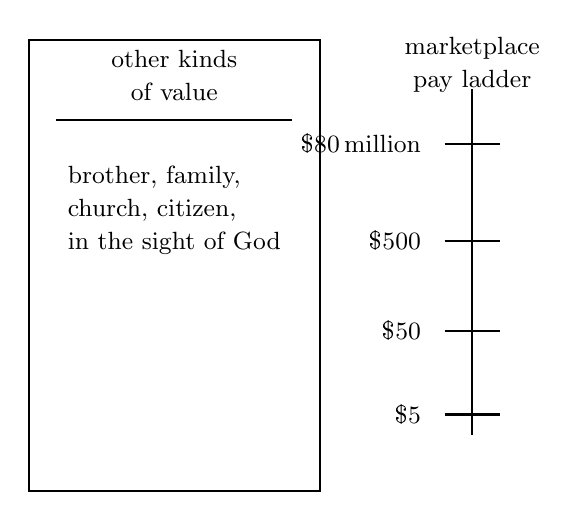
\begin{tikzpicture}[x=0.88cm,y=0.88cm]
\draw[thick] (0,0) rectangle (4.2,6.5);
\node[align=center] at (2.1,6.0) {\small other kinds\\\small of value};
\draw (0.4,5.35) -- (3.8,5.35);
\node[align=left] at (2.1,4.05) {\small brother, family,\\\small church, citizen,\\\small in the sight of God};

\draw[thick] (6.4,0.8) -- (6.4,5.8);
\draw[thick] (6.0,1.1) -- (6.8,1.1);
\draw[thick] (6.0,2.3) -- (6.8,2.3);
\draw[thick] (6.0,3.6) -- (6.8,3.6);
\draw[thick] (6.0,5.0) -- (6.8,5.0);

\node[left] at (5.8,1.1) {\small \$5};
\node[left] at (5.8,2.3) {\small \$50};
\node[left] at (5.8,3.6) {\small \$500};
\node[left] at (5.8,5.0) {\small \$80\,\text{million}};

\node[align=center] at (6.4,6.15) {\small marketplace\\\small pay ladder};
\end{tikzpicture}
\caption{Cautious redraw of the easel structure. The right ladder is the secure part. The left block is transcript-assisted and remains intentionally generic because the handwriting itself is not fully legible.}
\end{figure}

The board's top heading appears to concern value, but it is not secure enough to quote as exact text. The safer interpretive point comes from the transcript itself. Rohn immediately insists that marketplace valuation is not the same thing as total human worth:
\begin{equation}
\text{human/social value} \not\equiv \text{marketplace value}.
\end{equation}
A person may be valuable as a brother, in a family, in a church, as a citizen, and in the sight of God, yet still not be very valuable \emph{to the marketplace}. That distinction is crucial. The lecture wants the marketplace ladder, but it does not want moral reductionism.

Only after this restraint does the practical rule emerge in full clarity: work harder on yourself than you do on your job. We now know why that sentence appears here. The ladder has given the lecture a visible scale, and the lecture can now ask how one actually becomes the kind of person the marketplace values more highly.

\section{Experience, OPE, Books, and Journals}

Once the lecture has made its economic point, it deliberately broadens personal development into a method of learning. The rhythm changes. We are no longer moving up a ladder of pay; we are building a ladder of intake.

The sequence is cumulative:
\begin{enumerate}
\item personal experience,
\item OPE, other people's experiences,
\item observation,
\item listening,
\item reading,
\item journaling.
\end{enumerate}

The first layer is personal experience. We are to look back over the last months and years, identify what failed, and correct it. Mr.~Shouf's summary is almost comic in its severity: if what we are doing is not working, we should stop doing it. The lecture refuses to romanticize failure. Failure is useful only if it is converted into information.

The second layer is OPE. This is one of the lecture's better compact phrases, because it enlarges the student's field of evidence immediately. We are not trapped inside our own mistakes. We may learn from those who have done poorly and from those who have done well. The speaker jokes that failures rarely hold seminars, but the logical point is sound. There is no reason to pay full price for every lesson if another person's life has already exhibited the pattern.

This borrowed experience then branches into observation and listening. We watch disciplines at work; we listen to lectures, sermons, teachers, and tapes. The speaker is explicit that he wants this video itself to function in exactly that way: as an instance of other people's experience translated into usable form.

Reading comes next, and here the lecture becomes concrete again. Rohn names the Bible, \emph{Think and Grow Rich}, and \emph{The Richest Man in Babylon}. The content is less important than the method. Books extend the radius of experience. They allow other lives, and other summaries of life, to be carried into our own development.

Journaling is the final conversion step. The lecture's advice is practical and exact: do not trust memory; write down what matters. Even here there is a quiet update rule:
\begin{equation}
\text{heard or seen value} \longrightarrow \text{written note} \longrightarrow \text{later review} \longrightarrow \text{usable value}.
\end{equation}
The journal is therefore not ornament but storage. It is where transient impressions become retrievable substance.

This is the point at which the first subject closes. We have moved from marketplace pay to self-education, and the lecture is now ready for the second subject. The question becomes: what shall all this development be \emph{for}?

\section{Goals: Past as School, Future as Promise}

The second subject is goal-setting, but once again the lecture does not begin with technique. It begins by reorganizing time. First the past. The past is to be treated as a school, not a burden and not a weapon with which we beat ourselves. That is a conceptual reframing before it is a motivational one. The same past may either instruct or immobilize, depending on how it is classified.

Then the lecture turns to the future and gives it a new name. The future is the promise. This is the key transition. The talk is not yet listing goals; it is explaining why a future needs design at all.

\subsection{Question \& Answer}

\paragraph{Question.} Why do most people face the future with apprehension instead of anticipation?

\paragraph{Answer.} Because the future is usually left undesigned. The lecture's contrast is well captured by
\begin{equation}
\text{future not designed} \Rightarrow \text{apprehension}, \qquad
\text{future well designed} \Rightarrow \text{anticipation}.
\end{equation}

This is one of the strongest local tension-and-resolution beats in the lecture. The future by itself is not the frightening thing. What frightens is vagueness. When the future is made definite, it ceases to be merely a source of anxiety and becomes an attractive object of thought.

Only now does Rohn turn to procedure. The procedure is strikingly simple:
\begin{enumerate}
\item decide what we want,
\item write it down,
\item keep the old lists,
\item check things off.
\end{enumerate}
The simplicity is part of the pedagogy. The lecture is removing excuses. We do not need a sophisticated system to begin. We need seriousness, paper, and the willingness to be explicit.

The Spain anecdote belongs here, even though the transcript is rough in a few local details. The secure point is that Spain was once a written goal, and when the plane touched down in Madrid, it was checked off in the journal. The lecture wants the future to become concrete enough that realization has a visible mark.

Yet list-making by itself is not the end of the section. The lecture has one more move to make before turning to money again. It must explain why goals make discipline psychologically bearable.

\section{Promise, Price, and What Goals Make of Us}

At this stage the lecture prevents a common flattening. Goals are not only for getting things. They are also for becoming someone. Rohn makes those two claims inseparable.

The first claim is about promise and price. Every promise has a price. The price may be books, classes, habits, and disciplines, but the price must be paid. The lecture's compact law is
\begin{equation}
\text{promise clarity}\uparrow \Rightarrow \text{price difficulty}\downarrow.
\end{equation}
The price does not vanish. What changes is our willingness to bear it. A vague future makes discipline feel arbitrary. A clear future makes the same discipline intelligible.

This is why the lecture ties goal-setting back to personal development. A designed future does not merely specify outcomes; it stabilizes effort in the present. In that sense the goal is not the reward at the end of the process. It is also the device that allows the process to continue.

The lecturer then intensifies the point with the millionaire example. Mr.~Shouf urges the young Rohn to set a goal to become a millionaire, but not chiefly because a million dollars would be pleasant to possess. The deeper reason is what such a goal would require him to become. The talk later checks this claim against experience. By thirty-one he is a millionaire; by thirty-three he is broke. The money disappears, but the transformed person does not. The skills, the knowledge of the marketplace, the language, and the disciplines remain.

That is why Rohn says, in substance, that what makes us valuable is not what we get but what we become. The durable quantity is the enlarged self, not the temporary cash balance. Goals must therefore be large enough to demand growth, but not so distorted that they require the sale of character. The lecture insists on a middle road: high enough to stretch us, clean enough to keep us intact.

Only after this motivational correction does the third subject arrive. That order matters. Financial independence is introduced only after the lecture has explained why a financial plan can be carried without collapsing into mere greed.

\section{Financial Independence and the Dollar Formula}

Rohn now turns to the most formula-like part of the lecture. Even here he begins by choosing his terms carefully. He prefers the phrase \emph{financial independence} to the more emotionally charged language of becoming rich. That choice already tells us something about the lecture's structure: we are heading not toward display, but toward a condition of freedom.

\begin{definition}
Financial independence is the ability to live from the income of your own personal resources.
\end{definition}

The lecture immediately suggests a threshold condition:
\begin{equation}
\text{income from personal resources} \ge \text{required living expense}.
\end{equation}
This is a faithful companion reconstruction of the spoken definition. It should not be mistaken for finance theory. The lecture gives no rate calculations and no portfolio model. It gives a criterion: if resources generate enough income to support the chosen way of living, then independence has been reached in the lecture's sense.

The proposed horizon is equally plain:
\begin{equation}
15 \to 35 = 20\ \text{years}.
\end{equation}
The claim is that twenty years is enough time to become financially independent if one has the right plan. If the result fails to appear, the lecture says, we should inspect the plan before blaming the country.

That brings us to philosophy. The order of spending and investing is the decisive point:
\begin{align}
\text{poor philosophy} &: \text{spend first, invest what is left},\\
\text{rich philosophy} &: \text{invest first, spend what is left}.
\end{align}
The lecture explicitly says that the amount is not the main thing. The order is the main thing. Philosophy appears here not as abstraction, but as the rule that decides which operation comes first.

\subsection{Question \& Answer}

\paragraph{Question.} What should a child do with a dollar?

\paragraph{Answer.} The lecture's first answer is negative: do not spend it all. Only after that negative command does the positive allocation appear:
\begin{equation}
1.00 = 0.70 + 0.10 + 0.10 + 0.10.
\end{equation}
The three investment-side tenths are then named explicitly:
\begin{equation}
0.10 = \text{charity},\qquad
0.10 = \text{active capital},\qquad
0.10 = \text{passive capital}.
\end{equation}

\begin{table}[t]
\centering
\begin{tabular}{ll}
$0.70$ & spending \\
$0.10$ & charity \\
$0.10$ & active capital \\
$0.10$ & passive capital
\end{tabular}
\caption{The lecture's dollar-allocation rule. It is presented as a compact working discipline, not as a formal finance model.}
\end{table}

The first tenth is generosity. The lecture treats this not only as charity but as character formation. The second tenth is active capital, money set aside to produce profit directly. The third is passive capital, money put in the hands of others so that it yields interest. At that point the lecture names compound interest, but it does not derive a formula for it. We should keep the name and the qualitative role, and not pretend the lecture has done more than that.

The active-capital example is concrete enough to serve as a worked exercise:
\begin{align}
\text{purchase of broken wagon} &= \$1,\\
\text{sale after repair} &= \$5,\\
\text{profit} &= \$4.
\end{align}
This is small on purpose. The lecture wants capital formation to begin at child scale. A dollar is enough to begin the philosophy. The point is not the size of the project, but the habit of turning resources into profit rather than immediately dissolving them in consumption.

That is why the lecture states its wage-and-profit maxim so sharply:
\begin{equation}
\text{wages make a living},\qquad \text{profits make a fortune}.
\end{equation}
A compressed companion form is
\begin{equation}
\text{profits} > \text{wages}.
\end{equation}
Again, this is not a theorem in economics. It is a lecture ranking: wages are respectable and necessary, but profits are what scale.

The passive-capital side leads to the power relation:
\begin{equation}
\text{lender} > \text{borrower}.
\end{equation}
The spoken form is that the borrower is servant to the lender, and that the lender occupies the power position. The notation above is merely a compact rendering of that claim.

The lecture then refuses to let the section end as a mechanical budget lesson. It returns to attitude. Paying bills is reinterpreted as reducing liabilities. Paying taxes is placed inside a larger system that sustains the whole economic order, the famous goose that lays the golden eggs. Whether or not we agree with the rhetoric, the structural point is important: even a formula as simple as \(70/10/10/10\) will not hold without an attitude capable of carrying it.

\section{Summary}

The lecture begins with a broke twenty-five-year-old and ends with four questions. Between those points it builds a continuous path. First, the teacher's promise: change the self and the outcome changes. Next, the wind-and-sail model: conditions matter, but steering matters too. Then personal development begins with economics: pay is tied not to time alone but to value brought to the marketplace. From there the lecture broadens into learning by experience, observation, listening, reading, and journaling. Only then does it move to goals, to the design of the future, to the relation between promise and price, and finally to the dollar formula for financial independence.

The closing questions remain important because they are the lecture's final compression of the whole argument:
\begin{enumerate}
\item Why?
\item Why not?
\item Why not you?
\item Why not now?
\end{enumerate}
These are not proofs. They are activation points. The chapter's mathematics is therefore modest but real: a few definitions, a few comparison rules, a ladder, a time horizon, and a dollar split. Their purpose is not to build a science of economics. Their purpose is to make the lecture's practical sequence legible: self-change, deliberate learning, designed goals, disciplined allocation, and a future that is steered rather than merely awaited.